\section{Coordinate Systems}
\label{sec:Coord}

  The only material not covered here in full detail is the mathematical explanation of reference frames, for which one should see the reference papers. It suffices to summarize as follows: GEANE objects (matrices and parameter vectors) are defined and calculated in the Geant4 source code in the free particle system. Then there is an intermediate surface system defined in XYZ, as the Geant4 surface trajectory system must be defined in an orthogonal coordinate system, before which parameter objects are converted to the most natural detector system of XUV. (Important note - be very careful with coordinate system variables, letters are reused between different papers and code bases with different configurations and meanings constantly.)


Notes on coordinate systems I use - UV pointing outward vs XYZ, XUV x being forward, UVW in geante src, maybe IJK/TUV in one paper-prob not, GeaneTrackerWorld[0,12,18], rotateArcTracker (bit more specific), magnetic field access coordinates?, JacobianToUV
- this should be in coord sys file



\begin{figure}[]
\caption{Shown here is a picture of the 3 trackers in the world geometry in their approximate positions. First note the world coordinate system shown in the bottom left of the plot, where the origin lives at the center of the ring. Tracks are then generated and read out from the trackers in their three world positions in red. Due to the reconstruction bug where tracks improperly reconstruct if their momenta is too aligned with the globabl Z axis, the reconstruction rotates the entire arc including tracker 0 to the blue position, where planes are parallel in X, and this problem is avoided. Track parameters from the 3 positions are then rotated to this reference frame by the amounts shown on the plots for the reconstruction stage, and at the end are rotated back.}
\centering
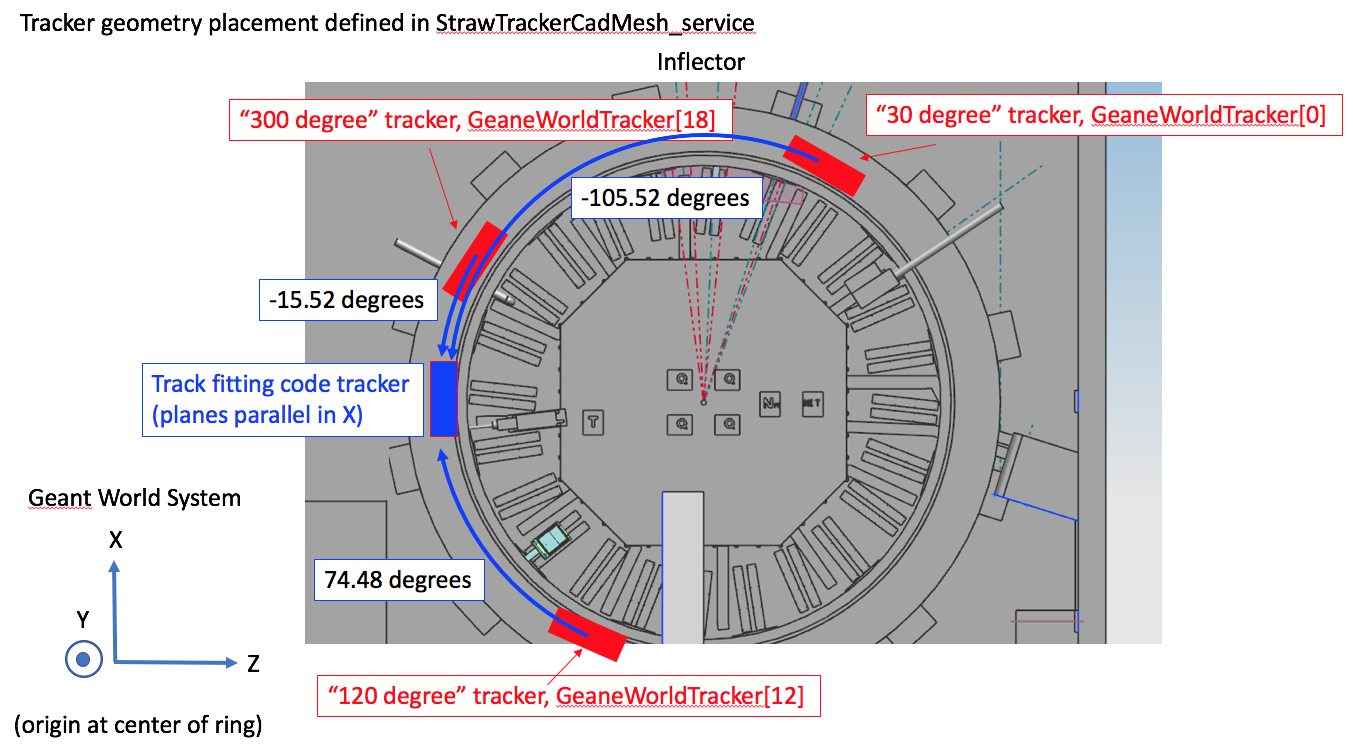
\includegraphics[width=1.0\textwidth]{WorldCoordSys}
\label{fig:WorldCoordSys}
\end{figure}

\begin{figure}[]
\caption{This picture shows the coordinate system in which the the Geane track reconstruction is performed, in relation to the world coordinate system. The origin remains at the center of the ring, with the tracking planes parallel in X in the reconstruction, going forward in number. Y is vertically up, and Z is horizontally to the right. U and V are defined such that they have greater values with higher radii and increasing straw number.}
\centering
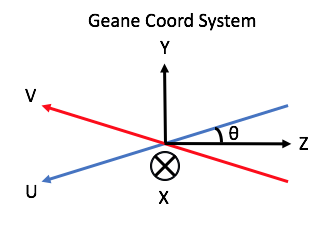
\includegraphics[width=0.6\textwidth]{GeaneCoordSys}
\label{fig:GeaneCoordSys}
\end{figure}


$1/p, \lambda, \phi, y_{\perp}, z_{\perp}$, free system

$1/p, py/px, pz/px, y, z$, surface system

$
\begin{pmatrix}
u \\
v \\
\end{pmatrix} =
\begin{pmatrix}
-\sin{\theta} & -\cos{\theta} \\
\sin{\theta} & -\cos{\theta} \\
\end{pmatrix}
\begin{pmatrix}
y \\
z \\
\end{pmatrix}
$, yz to uv matrix, where $\theta$ is $7.5\degree$, the 5x5 transformation is just a 1 in the top left corner, and then this matrix in the remaining 2 diagonal blocks

$1/p, pu/px, pv/px, u, v$, uv system




Secondly, the RunGeane.fcl file loads all 3 trackers necessary for symbol and name definitions, but such that tracker 0 (or 18) is rotated such that the tracking planes are parallel to the global geant X axis (using the rotateArcTracker fcl parameter for the Arc service). This is done to avoid the issue of error propagation instability close to the Z axis, as detailed in \href{http://gm2-docdb.fnal.gov:8080/cgi-bin/ShowDocument?docid=4567}{DocDB 4567}, while at the same time still observing the correct azimuthally symmetric 2D field for the tracks.
